\chapter{Грамматическое описание языка}\label{appendix-MikTeX-TexStudio}							% Заголовок
%\addcontentsline{toc}{chapter}{Second call for chapters to participate in the book Machine learning in analysis of biomedical and socio-economic data}	% Добавляем его в оглавление

Далее представлена грамматика языка охраняемых команд в расширенной форме Бэкуса-Наура.
Метасимволы РБНФ выделены красным цветом, а терминальные цепочки самого языка охраняемых команд
выделены синим цветом.
\begin{Verbatim}[commandchars=\\\{\}]
<программа> ::= <список операторов> <список макро-функций>
<список операторов> ::= <оператор> \textcolor{red}{\{} \textcolor{blue}{;} <оператор> \textcolor{red}{\}}
<оператор> ::= <оператор присваивания> \textcolor{red}{|} <условный оператор> \textcolor{red}{|} 
    <оператор цикла> \textcolor{red}{|} <вызов макро-функции>
<оператор присваивания> ::= <идентификатор> \textcolor{blue}{:=} <выражение> \textcolor{red}{|}
    <идентификатор> <оператор присваивания> <выражение>
<цифра> ::= \textcolor{blue}{0} \textcolor{red}{|} ... \textcolor{red}{|} \textcolor{blue}{9}
<число> ::= <цифра> \textcolor{red}{\{}<цифра>\textcolor{red}{\}} \textcolor{red}{[} \textcolor{blue}{.} <цифра> {<цифра>} \textcolor{red}{]}
<буква> ::= \textcolor{blue}{_} \textcolor{red}{|} \textcolor{blue}{a} \textcolor{red}{|} ... \textcolor{red}{|} \textcolor{blue}{z} \textcolor{red}{|} \textcolor{blue}{A} \textcolor{red}{|} ... \textcolor{red}{|} \textcolor{blue}{Z}
<идентификатор> ::= <буква> \textcolor{red}{\{}<буква> \textcolor{red}{|} <цифра>\textcolor{red}{\}}
<выражение> ::= <идентификатор> \textcolor{red}{|} <число> \textcolor{red}{|} \textcolor{blue}{True} \textcolor{red}{|} \textcolor{blue}{False} \textcolor{red}{|}
    \textcolor{blue}{(}<выражение>\textcolor{blue}{)} \textcolor{red}{|} \textcolor{blue}{-}<выражение> \textcolor{red}{|} \textcolor{blue}{~}<выражение> \textcolor{red}{|}
    <выражение> \textcolor{blue}{+} <выражение> \textcolor{red}{|} <выражение> \textcolor{blue}{-} <выражение> \textcolor{red}{|}
    <выражение> \textcolor{blue}{*} <выражение> \textcolor{red}{|} <выражение> \textcolor{blue}{/} <выражение> \textcolor{red}{|}
    <выражение> \textcolor{blue}{&} <выражение> \textcolor{red}{|} <выражение> \textcolor{blue}{|} <выражение> \textcolor{red}{|}
    <выражение> \textcolor{blue}{==} <выражение> \textcolor{red}{|} <выражение> \textcolor{blue}{!=} <выражение> \textcolor{red}{|}
    <выражение> \textcolor{blue}{>} <выражение> \textcolor{red}{|} <выражение> \textcolor{blue}{>=} <выражение> \textcolor{red}{|}
    <выражение> \textcolor{blue}{<} <выражение> \textcolor{red}{|} <выражение> \textcolor{blue}{<=} <выражение> \textcolor{red}{|}
    <выражение> \textcolor{blue}{>>} <выражение>
<охраняемая команда> ::= <выражение> \textcolor{blue}{->} <список операторов>
<список охраняемых команд> ::= <охраняемая команда> 
    \textcolor{red}{\{} \textcolor{blue}{|} <охраняемая команда>\textcolor{red}{\}}
<условный оператор> ::= \textcolor{blue}{if} <список охраняемых команд> \textcolor{blue}{fi}
<оператор цикла> ::= \textcolor{blue}{do} <список охраняемых команд> \textcolor{blue}{od}
<список макросов> ::= \textcolor{red}{\{}<определение макро-функции>\textcolor{red}{\}}
<определение макросов> ::= <идентификатор>  
    \textcolor{blue}{(} \textcolor{red}{[}<идентификатор> \textcolor{red}{\{}, <идентификатор>\textcolor{red}{\}}\textcolor{red}{]} \textcolor{blue}{)} \textcolor{blue}{:=} <список операторов>
<вызов макроса> ::= <идентификатор> 
    \textcolor{blue}{(} \textcolor{red}{[}<выражение> \textcolor{red}{\{}, <выражение>\textcolor{red}{\}}\textcolor{red}{]} \textcolor{blue}{)}
\end{Verbatim}

% %\chapter{\normalfont\normalsize{}Часто задаваемые вопросы (FAQ)}\label{Appendix-FAQ}							% Заголовок
% %%\addcontentsline{toc}{chapter}{Second call for chapters to participate in the book Machine learning in analysis of biomedical and socio-economic data}	% Добавляем его в оглавление


% Далее приведены формулы \eqref{eq:Pi-app2}, \eqref{eq:Pi-app2-},  \firef{fig:spbpu_hydrotower-app2}, \firef{fig:spbpu_hydrotower-app2-}, \taref{tab:ToyCompare-app2}, \taref{tab:ToyCompare-app2-}.


% \begin{equation}% лучше не оставлять пропущенную строку (\par) перед окружениями для избежания лишних отсупов в pdf
% \label{eq:Pi-app2-} % eq - equations, далее название, ch поставлено для избежания дублирования
% \pi \approx 3,141.
% \end{equation}

% %
% \begin{figure}[ht!] 
% 	\center
% 	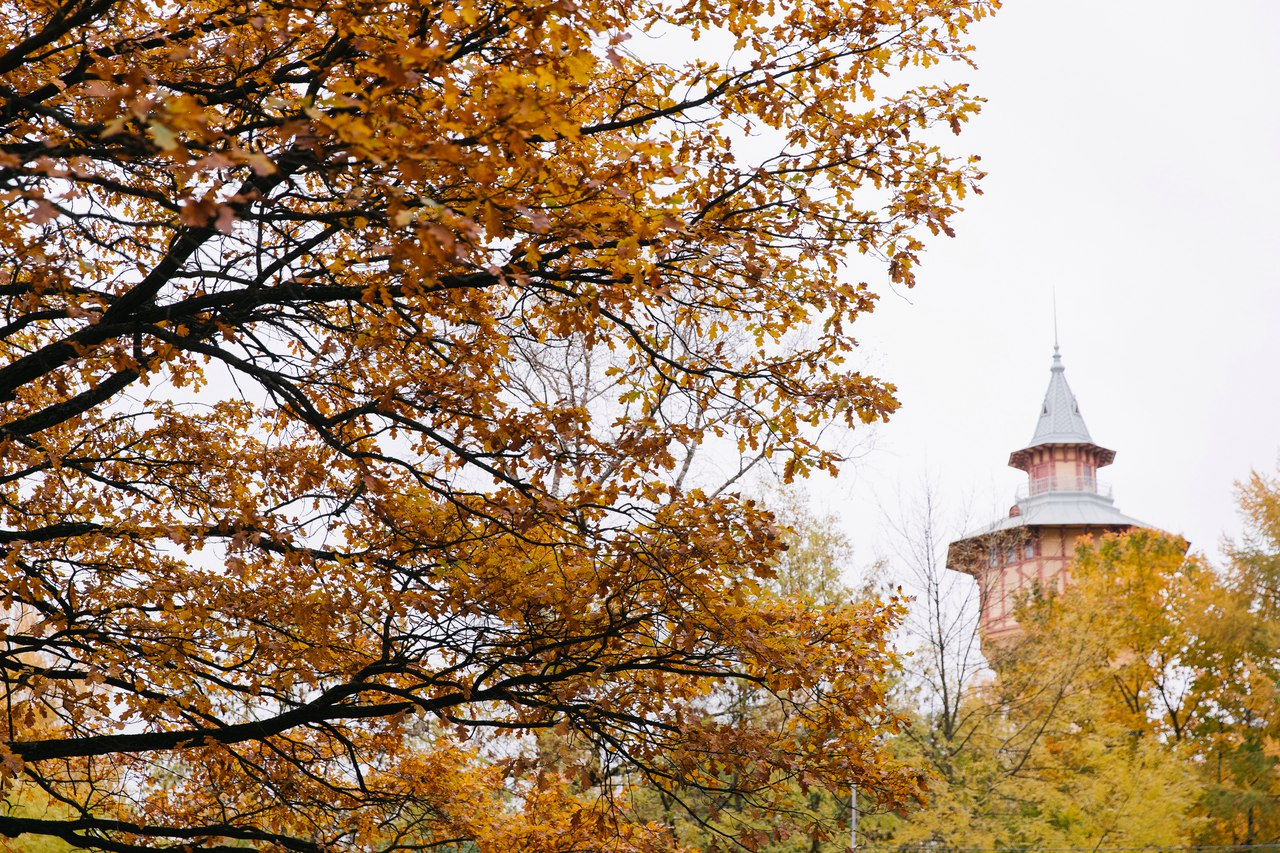
\includegraphics [scale=0.27] {my_folder/images//spbpu_hydrotower}
% 	\caption{Вид на гидробашню СПбПУ \cite{spbpu-gallery}} 
% 	\label{fig:spbpu_hydrotower-app2-}  
% \end{figure}

% \begin{table} [htbp]% Пример оформления таблицы
% 	\centering\small
% 	\caption{Представление данных для сквозного примера по ВКР \cite{Peskov2004}}%
% 	\label{tab:ToyCompare-app2-}		
% 	\begin{tabular}{|l|l|l|l|l|l|}
% 		\hline
% 		$G$&$m_1$&$m_2$&$m_3$&$m_4$&$K$\\
% 		\hline
% 		$g_1$&0&1&1&0&1\\ \hline
% 		$g_2$&1&2&0&1&1\\ \hline
% 		$g_3$&0&1&0&1&1\\ \hline
% 		$g_4$&1&2&1&0&2\\ \hline
% 		$g_5$&1&1&0&1&2\\ \hline
% 		$g_6$&1&1&1&2&2\\ \hline		
% 	\end{tabular}	
% 	\normalsize% возвращаем шрифт к нормальному
% \end{table}




% \section{Параграф приложения}\label{app-2-1}							


% \subsection{Название подпараграфа} \label{ch2:subsec-title-abbr} %название по-русски


% Название подпараграфа оформляется с помощью команды  \texttt{\textbackslash{}subsection\{...\}}.

% Использование подподпараграфов в основной части крайне не рекомендуется.
% \subsubsection{Название подподпараграфа}\label{ch2:subsubsec-title-abbr} %название по-русски

% \begin{equation}% лучше не оставлять пропущенную строку (\par) перед окружениями для избежания лишних отсупов в pdf
% \label{eq:Pi-app2} % eq - equations, далее название, ch поставлено для избежания дублирования
% \pi \approx 3,141.
% \end{equation}
% %
% %
% \begin{figure}[ht!] 
% 	\center
% 	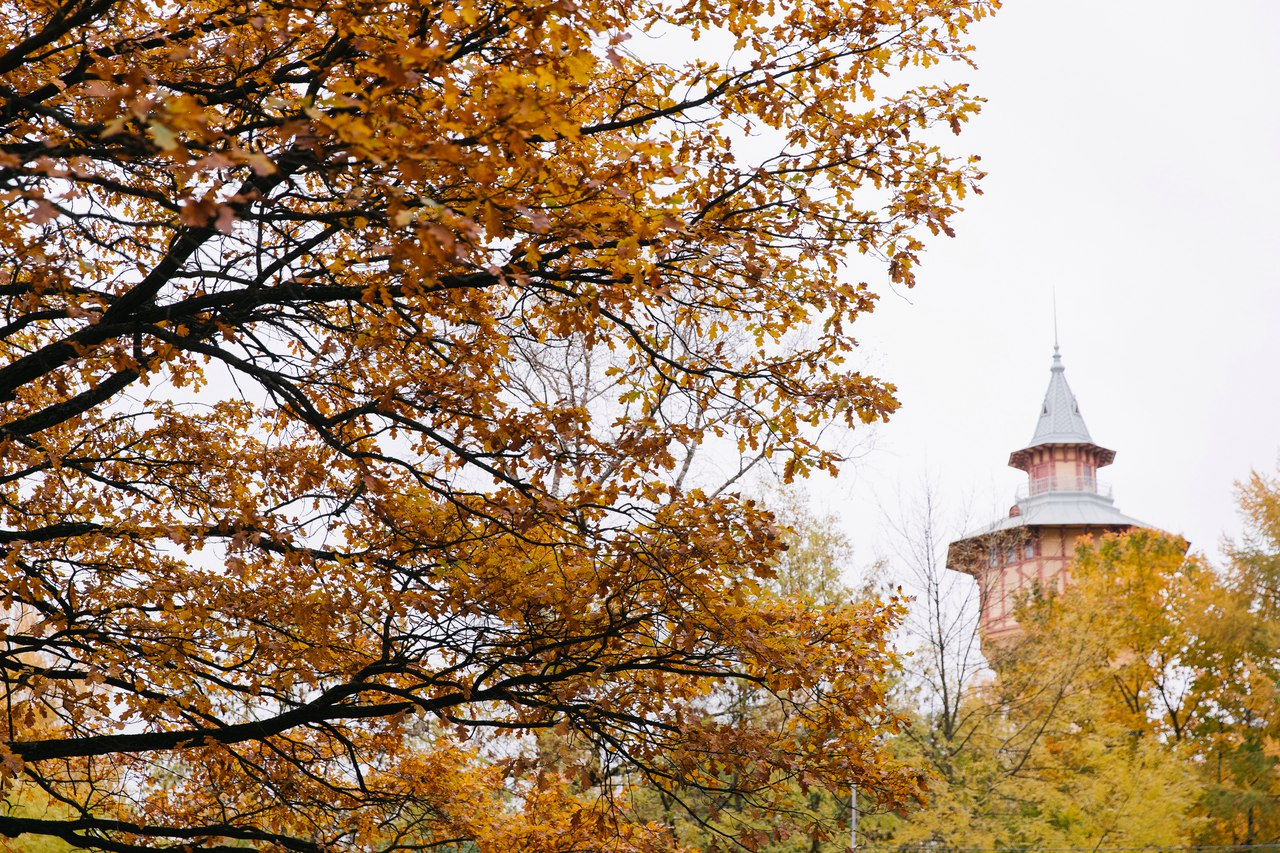
\includegraphics [scale=0.27] {my_folder/images//spbpu_hydrotower}
% 	\caption{Вид на гидробашню СПбПУ \cite{spbpu-gallery}} 
% 	\label{fig:spbpu_hydrotower-app2}  
% \end{figure}
% %




% \begin{table}[t!]% Пример оформления таблицы
% 	\centering\small
% 	\caption{Представление данных для сквозного примера по ВКР \cite{Peskov2004}}%
% 	\label{tab:ToyCompare-app2}		
% 	\begin{tabular}{|l|l|l|l|l|l|}
% 		\hline
% 		$G$&$m_1$&$m_2$&$m_3$&$m_4$&$K$\\
% 		\hline
% 		$g_1$&0&1&1&0&1\\ \hline
% 		$g_2$&1&2&0&1&1\\ \hline
% 		$g_3$&0&1&0&1&1\\ \hline
% 		$g_4$&1&2&1&0&2\\ \hline
% 		$g_5$&1&1&0&1&2\\ \hline
% 		$g_6$&1&1&1&2&2\\ \hline		
% 	\end{tabular}	
% 	\normalsize% возвращаем шрифт к нормальному
% \end{table}


%% В случае, когда таблица (рисунок) размещаются на последней странице, для переноса названия приложения на новую строку используем:
\NewPage % начать новое приложение с новой страницы 